\documentclass[10pt,a4paper]{article}
\usepackage[utf8]{inputenc}
\usepackage[english]{babel}
\usepackage[left=2cm,right=2cm,top=2cm,bottom=2cm]{geometry}
\usepackage[hyphens]{url}
\usepackage{hyperref}
\usepackage{listings}
\usepackage{color}
\usepackage{graphicx}
\graphicspath{{Figures/}}
\author{Pierre Lecomte \\ \textit{ \href{mailto:pierre.lecomte@gadz.org}{pierre.lecomte@gadz.org}}}
\title{ambitools Documentation}

%%% MY COLORS
\definecolor{yoheader}{rgb}{0.71,0.01,0.0}

%%%% margin par
\definecolor{margincolor}{rgb}{0.52,0.02,0.02} % grey red.
\definecolor{yobg}{rgb}{0.9,0.9,1}
\definecolor{yotxt}{rgb}{0.01,0.01,0.52}
\definecolor{mylstcmt}{rgb}{0.01,0.52,0.01} % a dark green.
%\definecolor{mylstdoc}{rgb}{0.60,0.60,0.60} % a medium grey.
\definecolor{mylstdoc}{rgb}{0.80,0.30,0.80} % a medium pink.
%\definecolor{mylsteqn}{rgb}{0.80,0.80,0.30} % a medium pink.
\definecolor{mylstkey}{rgb}{0.52,0.01,0.01} % a dark red.
%%\newcommand{\farg}[1]{\textrm{\textit{#1}}}

\begin{document}

\lstset{
  tabsize=4,
  showspaces=false,
  showstringspaces=false,
  %language=C++, 
  basicstyle=\ttfamily\color{yotxt},
  numbers=none,
  stepnumber=2,
  commentstyle=\slshape\color{mylstcmt},
  breaklines=true, 
  emph={component, declare, environment, import, library, process},
  emph={[3]button, checkbox, vslider, hslider, nentry, vgroup, hgroup, tgroup, vbargraph, hbargraph, attach},
  emphstyle=\color{mylstkey},
%  morecomment=[s][\color{mylsteqn}]{<equation>}{</equation>},
  morecomment=[s][\color{mylstdoc}]{<mdoc>}{</mdoc>},
  %% frame=single,
  backgroundcolor=\color{yobg},
  captionpos=b
}

\makeatletter
\newcommand\footnoteref[1]{\protected@xdef\@thefnmark{\ref{#1}}\@footnotemark}
\makeatother

\maketitle
\tableofcontents
\section{Introduction}

\subsection{Goals of ambitools}
ambitools is a collection of tools for sound-field synthesis using Near-Field Compensated Higher Orders Ambisonics (NFC-HOA). For the rest of this document, the denomination Ambisonics will be used for simplicity.

ambitools is developped in the context of my PhD on 3D sound field synthesis. The audio processing is coded in \textsc{Faust}\footnoteref{faustlive} (Functional AUdio Stream) which allows to produce efficent C++ code and exports in various DSP tools format : VST, standalone applications, lv2, etc. Thus, ambitools is multi-platform (although conceived under Linux/Jack).

The goal of ambitools is mainly to produces several modules to encode, decode and transform 3D synthesized sound field or 3D recordings in a context of physical sound field synthesis. 

The project is open-source under GPL licence. The \textsc{Faust} code is easily editable without beeing an C++ DSP engineer, so if a module should be adapted to a configuration, it'll be very easy to change a few lines in the code and produce quickly the required tool, using for example \textsc{FaustLive}\footnote{\label{faustlive}\url{http://faust.grame.fr}}.

Don't hesitate to contact me for any suggestions, requirements, critics or even just to tell me you're using ambitools !

\begin{flushright}
Pierre Lecomte
\end{flushright}

\subsection{Ambisonics}
This section presents the basis of Ambisonics for 3D sound field synthesis. If you're familiar with Ambisonics you may skip this section.

\section{Installing ambitools}

\subsection{Retrieve ambitools repository}
To install ambitools, simply go on the github repository\footnote{\url{https://github.com/sekisushai/ambitools}} and clone it. To do so, open a terminal in the directory you'd like to clone the repository and type the following command:

\begin{lstlisting}
$ git clone https://github.com/sekisushai/ambitools
\end{lstlisting}

To keep the repository up to date, type the following command at the root of the directory \lstinline`ambitools/`:

\begin{lstlisting}
$ git pull
\end{lstlisting}

You can also download a \lstinline'.zip' file from github\footnote{\url{https://github.com/sekisushai/ambitools/archive/master.zip}}

The resulting \lstinline'ambitools/' folder should have the following structure:

\begin{itemize}
    \item \lstinline'Documentation/' Everything concerning the documentation (pdfs, including some scientific papers).
    \item \lstinline'Faust/' Everything written in \textsc{Faust} language (all the ambitools plug-ins + some utilities).
    	\subitem \lstinline'bin/' Compiled plug-ins in various formats.
    	\subitem \lstinline'src/' Source code of the plug-ins.
    	\subitem \lstinline'src/lib/' Shared libraries.
    \item \lstinline'FIR/' Finite Impulse Response (FIR) filters banks for binaural rendering and spherical microphone equalization filters, to use with Jconvoler\footnote{\url{http://kokkinizita.linuxaudio.org/linuxaudio/}}, fast convolution software.
    	\subitem \lstinline'spherical_microphones/' Equalization filters for rigid spherical microphone, such as mh acoustics EigenMike\textsuperscript{\textregistered}\footnote{\url{http://www.mhacoustics.com}}
  		\subitem \lstinline'hrir/' Head Related Impulses Responses (HRIR) for various configurations to use with binaural rendering over headphones.
    \item \lstinline'Processing/' Everything written in \textsc{Processing} language, namely the spherical VU-Meter.
    	 \subitem \lstinline'bin/' Compiled spherical VU-Meter in Java for various architectures.
    	 \subitem \lstinline'src/' \textsc{Processing} source code.
    \item \lstinline'PureData/' Everything written in Pure Data (a few sounds generator patches, and PlayStation-like remote patch to drive \textsc{Faust} plug-ins with Open Sound Control protocol, OSC).
\end{itemize}

\subsection{Compile the \textsc{Faust} plug-ins}
The \textsc{Faust} plug-ins source codes are in the sub-folder \lstinline'Faust/src/'. 

\subsection{Local \textsc{Faust} compiler}
If you have \textsc{Faust} installed on your machine with the required dependencies, you can run the scripts collection \lstinline'faust2*' to produce the plug-in of your choice in the desired format. 

For example, to compile \lstinline'hoa_encoder.dsp' into a standalone Linux jack-qt application with \textsc{OSC} support, type the following command in a terminal in the folder \lstinline'\Faust/src'

\begin{lstlisting}
$ faust2jaqt hoa_encoder.dsp -osc
\end{lstlisting}

\subsection{\textsc{FaustLive}}
To compile the plug-ins to your requirements, load the chosen plug-in in \textsc{FaustLive}\footnoteref{faustlive} and choose "Window/Export As..." (see Fig.~\ref{fig:faustlive}).
\begin{figure}[!ht]
\centering
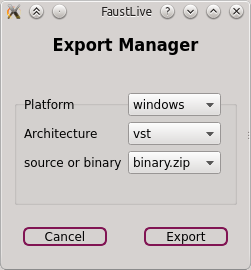
\includegraphics[width=0.3\columnwidth]{faustlive_export_manager.png}
\caption{\textsc{FaustLive} Export Manager}
\label{fig:faustlive}
\end{figure}

\subsection{Compile the \textsc{Processing} VU-Meter}
The \textsc{Processing} source code is in the folder \lstinline'Processing/scr'. You should open the file \lstinline'Spherical_VU_Meter.pde' in the \textsc{Processing} editor and select "File/Export..." to produce a binary application.

\section{The different tools}
This section gives a quick presentation of each tool contained in ambitools. 
\subsection{\textsc{Faust}}
The core of the sound processing is written in \textsc{Faust} language. Note that the majority of the figures presented here will be screenshots of the tools compiled as standalone \textsc{Jack} applications for Linux. However, thanks to the versatility of \textsc{Faust} compiler each of these tools can be compiled for various architecture, using \textsc{FaustLive}\footnoteref{faustlive} for example. 

\pagebreak
\subsubsection{hoa\_encoder}
\label{sec:hoa_encoder}
This first tool allows to encode a monophonic signal as 3D $B$-format spatial audio signals. The graphical user interface using Faust Linux jack-qet compiler is shown in Fig.~\ref{fig:hoa_encoder}. Two types of sources encoding are available : plane waves sources and spherical wave source. 

For the plane wave case, the check-box 'Spherical Wave Encoding' should be unselected. Consequently, the sliders 'Source Radius' and input entry 'Speaker Radius' are without effect on $B$-Format outputs signals.

For the spherical wave case, near-field filters are activated. \cite{daniel2003spatial,lecomte2015real}. Those filters use the decoding near-field compensation filters to be stable. Thus in this case, the radius of the spherical loudspeakers layout should be known prior to decoding. Consequently, the slider 'Source Radius' allows to choose the source radius to origin and the 'Speaker Radius' input entry fixes the loudspeakers radius to origin. At the decoding stage, using \lstinline'hoa_decoder' tools, the near-field compensation filters should be deactivated as they are already used at the encoding (see Sec.\ref{sec:hoa_decoder}).

\begin{figure}[!ht]
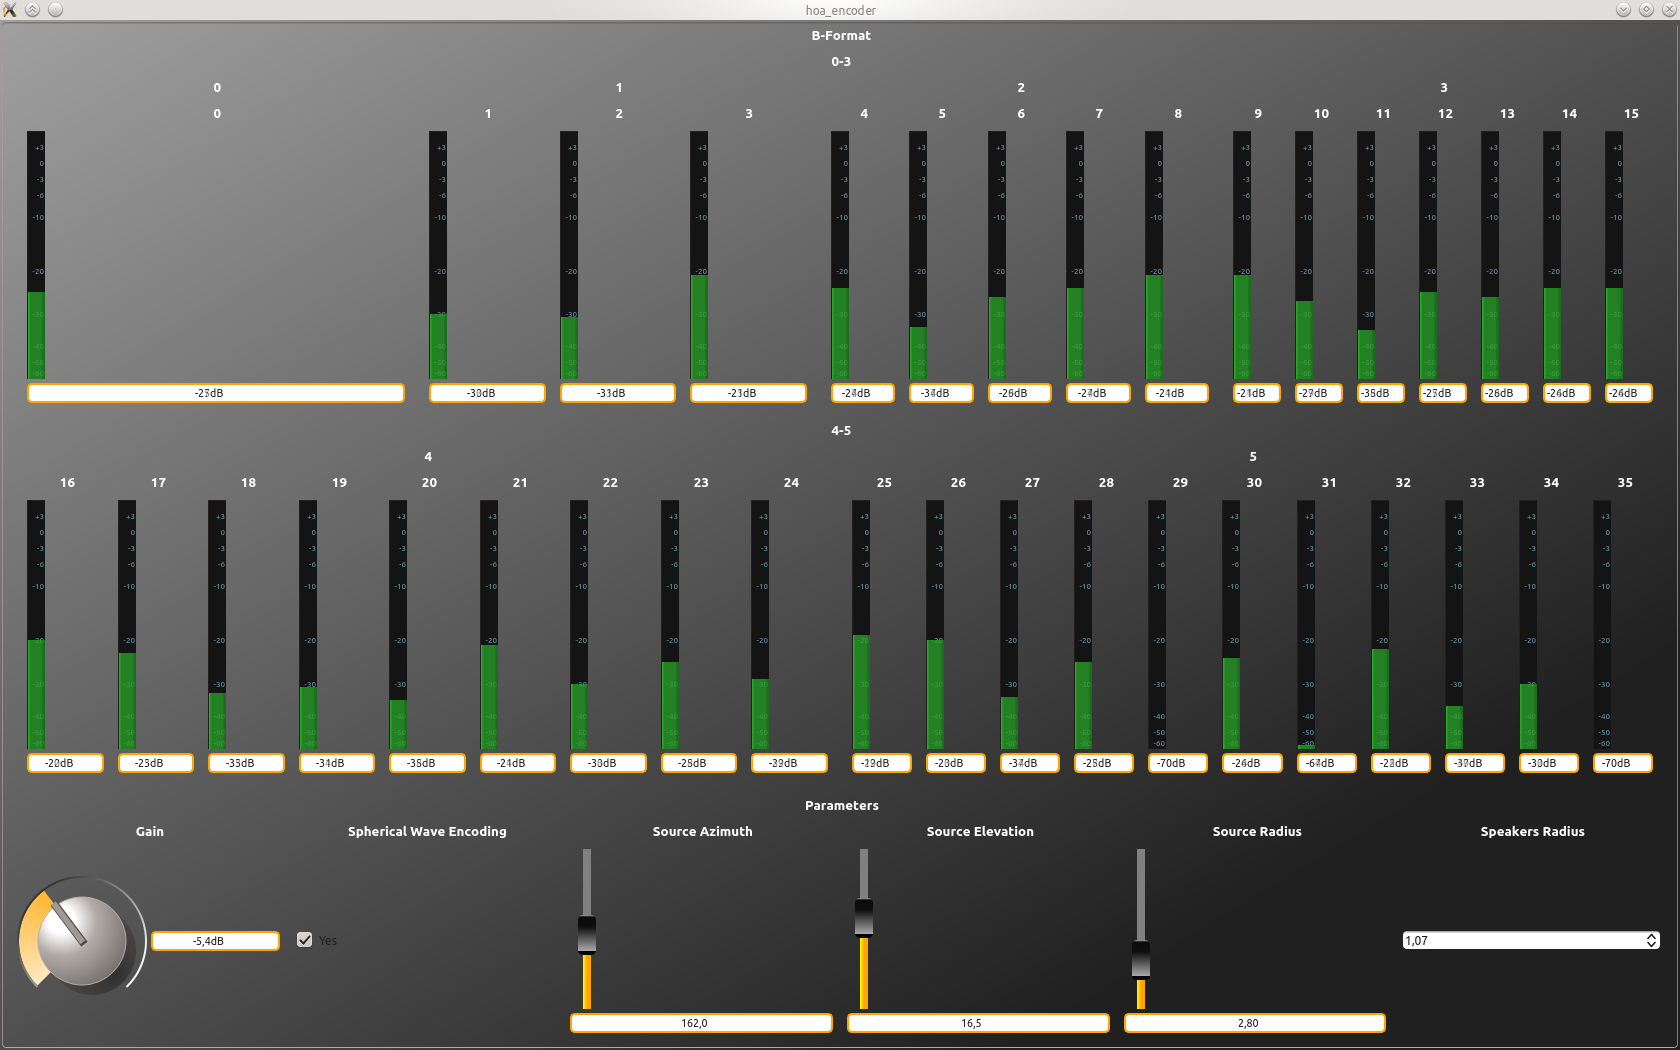
\includegraphics[width=\columnwidth]{hoa_encoder.png}
\caption{\lstinline'hoa_encoder' plug-in under linux jack-qt4. The 'Gain' button allows to adjust the input level of monophonic signal. The 'Spherical Wave Encoding' check-box enables the encoding of spherical wave, using near-field filters. 'Source Azimuth' and 'Source Elevation' sliders allows to choose the source direction. 'Source Radius' allows to choose the source distance to origin in case of spherical wave encoding. 'Speakers Radius' sets the radius for the spherical arrays of loudspeakers at decoding stage in case of spherical wave encoding. Finally the B-Format VU-Meters shows the level of 3D $B$-Format signals in dBFS up to order 5 (36 signals).}
\label{fig:hoa_encoder}
\end{figure}

\pagebreak
\subsubsection{hoa\_decoder\_*}
\label{sec:hoa_decoder}
Two basic decoder by mode matching \cite{daniel2000representation,poletti2005three} are available at the moment in ambitools: \lstinline'hoa_decoder_lebedev26' and
\lstinline'hoa_decoder_lebedev50'. Those two decoder allows to decode a $B$-Format on Lebedev grids with respectively 26 and 50 loudspeakers \cite{lebedev1975values,lecomte2015on}. Those grids are able to reconstruct the sound field up to order $3$ and $5$ respectively.
If other decoder are required, you should have a look at the ambisonic decoder toolbox from Aaron Heller \cite{heller2012toolkit}, or contact me. The graphical user interface using \textsc{Faust} Linux jack-qt compiler is shown in Fig.~\ref{fig:hoa_decoder_lebedev50} for the \lstinline'hoa_decoder_lebedev50' decoder. The decoder can be with or without near-field compensation (NFC) filters \cite{daniel2003further,lecomte2015real}. Those filters allow to take into account the finite distance of the loudspeakers : if they are disabled, the loudspeakers are seen as plane-wave generators. In case of spherical wave encoding using the \lstinline'hoa_encoder' plug-in, the filters should be disabled as the near-field compensation filters are already used at encoding step (see Sec.~\ref{sec:hoa_encoder}).
\begin{figure}[!ht]
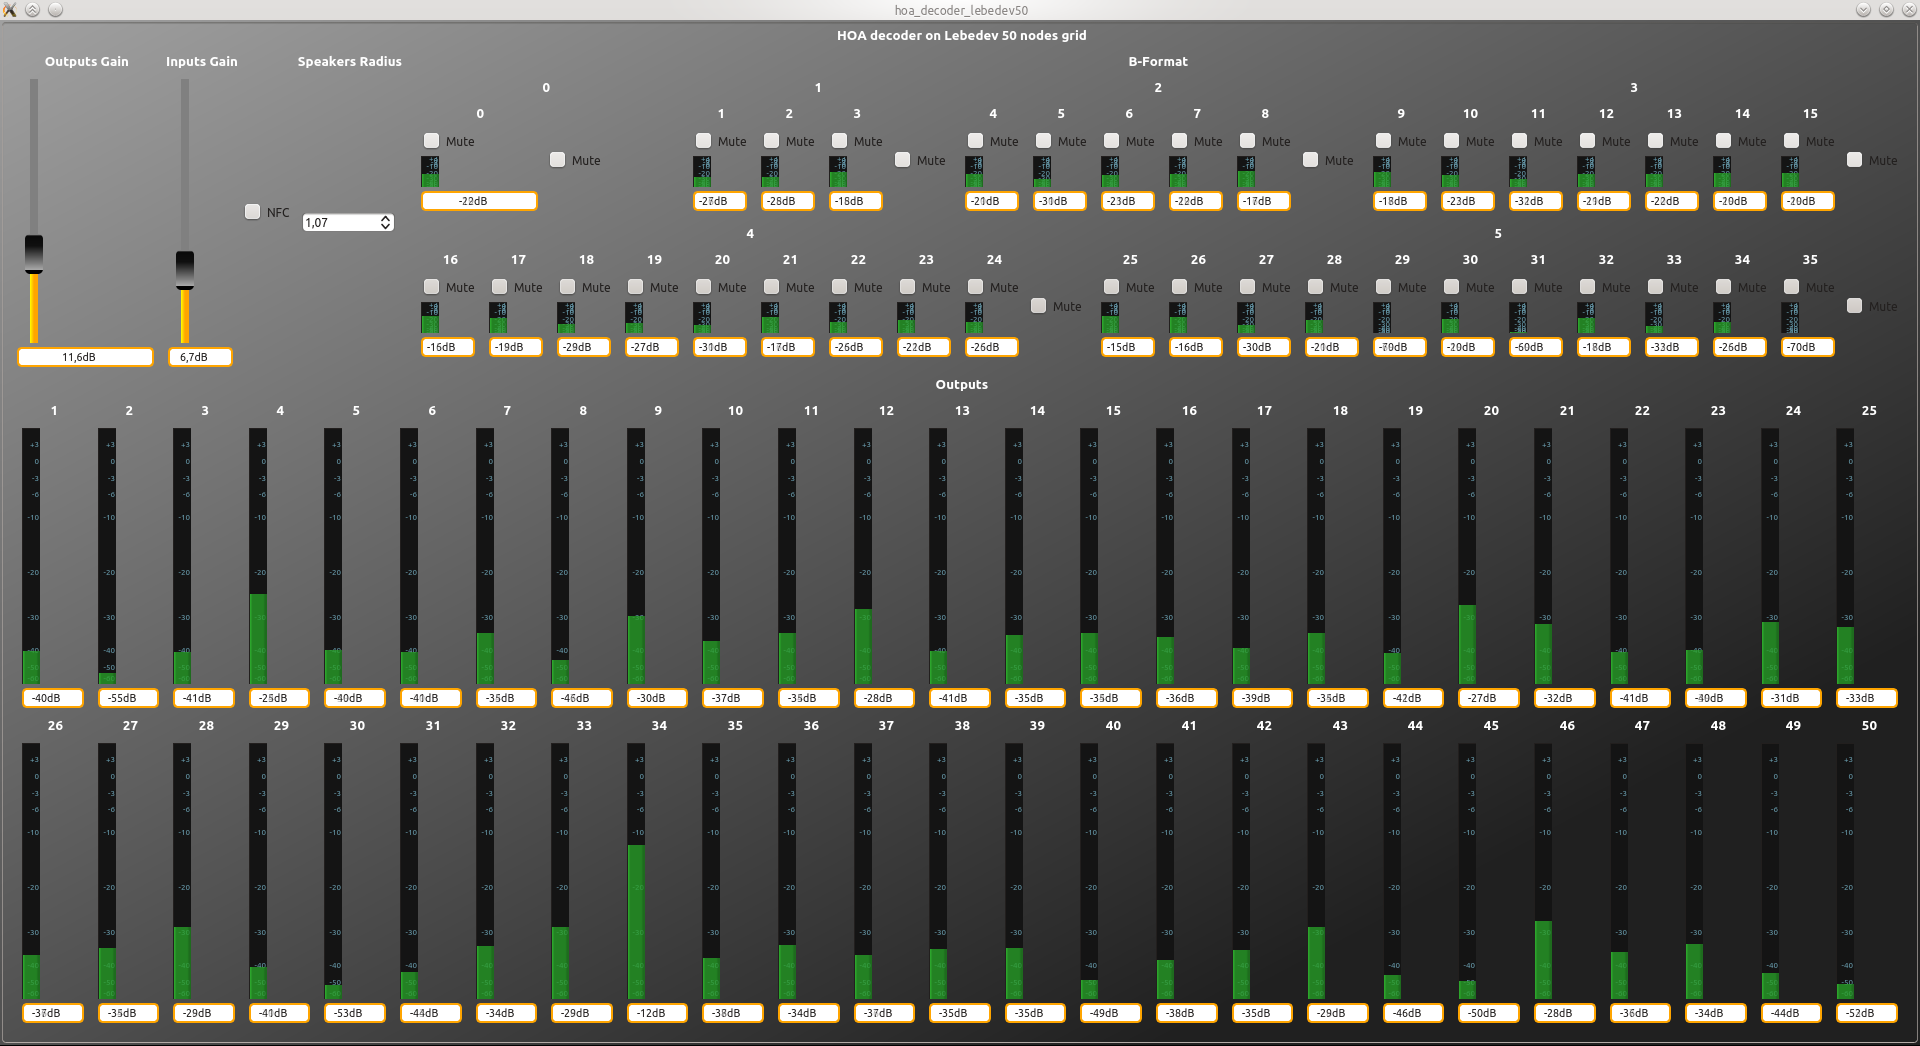
\includegraphics[width=\columnwidth]{hoa_decoder_lebedev50.png}
\caption{\lstinline'hoa_decoder_lebedev50' plug-in under linux jack-qt4. The slider 'Outputs Gain' apply a global gain on all outputs (loudspeakers signals). The slider 'Inputs Gain' apply a global gain on all inputs ($B$-Format signals). The VU-Meters 'Inputs' and 'Outputs' give the signal level in dBFS. The check-box 'NFC' activate or deactivate the near-field compensation filters. The input entry 'Speakers Radius' allows to set the spherical grid radius. Finally, the check-boxes 'Mute' above all inputs VU-meters allow to mute some specific $B$-Format signals. Or, all the signal from an order with 'Mute' check-boxes on side of an VU-Meter group.}
\label{fig:hoa_decoder_lebedev50}
\end{figure}

\pagebreak
\subsubsection{hoa\_panning\_*}
\label{section:hoa_panning}
It is possible to compute directly the driving signals of the loudspeakers without passing by and encoding/decoding process \cite{lecomte2015on}. This equivalent 3D panning is implemented in the tools \lstinline'hoa_panning_lebedev26' and \lstinline'hoa_panning_lebedev50' for 26 and 50 loudspeakers Lebedev grids respectively.
The graphical user interface using \textsc{Faust} Linux jack-qt compiler is shown in Fig.~\ref{fig:hoa_panning_lebedev50} for the \lstinline'hoa_panning_lebedev50' tool. For this version, two spherical waves are synthesized.
\begin{figure}[!ht]
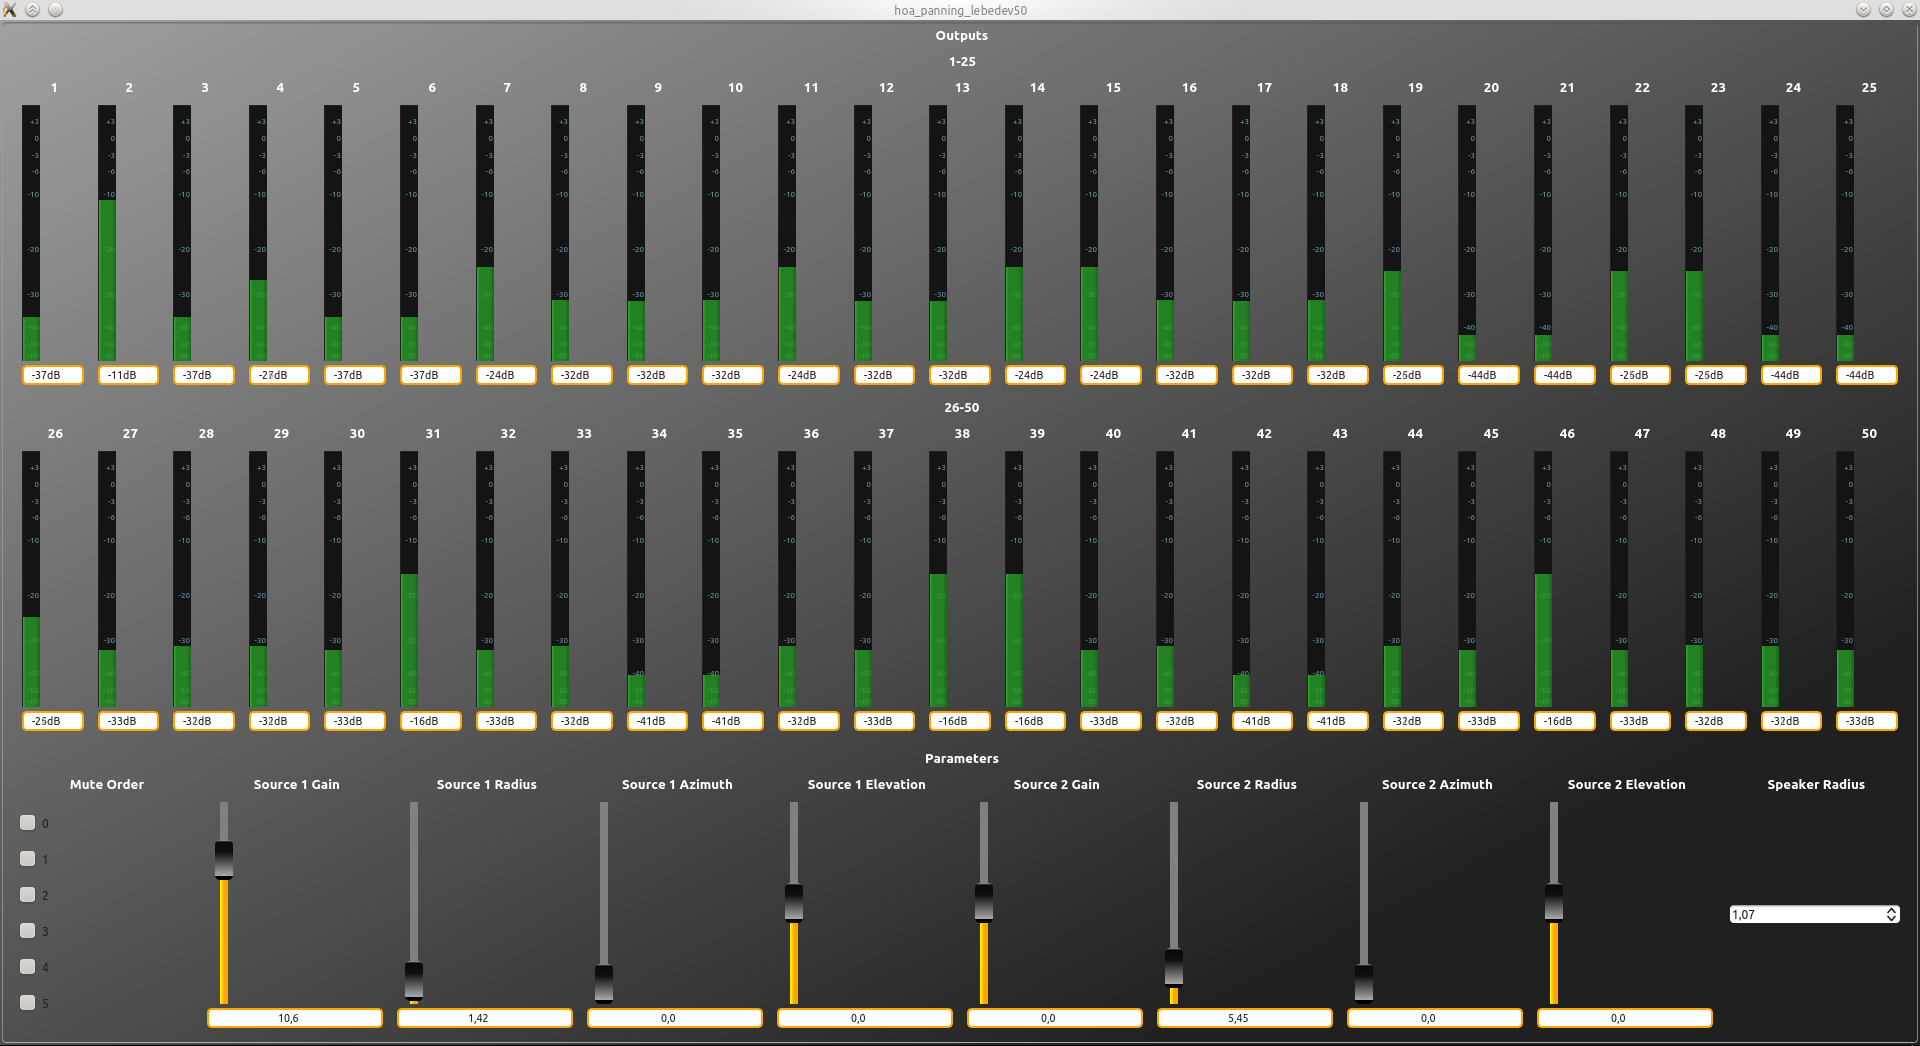
\includegraphics[width=\columnwidth]{hoa_panning_lebedev50.png}
\caption{\lstinline'hoa_panning_lebedev50' plug-in under Linux jack-qt4. The slider 'Outputs Gain' apply a global gain on all outputs (loudspeakers signals). The check-boxes 'Mute Order' allows to mute some Ambisonic orders in the computation of the driving signals. The sliders 'Gain' 'Radius' 'Azimuth' 'Elevation' controls the position and gain of two sources (spherical waves). In order to stabilize the near-field filters for spherical wave synthesis, the input entry 'Speaker Radius' fixes the loudspeaker array radius.}
\label{fig:hoa_panning_lebedev50}
\end{figure}

\pagebreak
\subsubsection{hoa\_mirroring}
The plug-in \lstinline'hoa_mirroring' allows a sound field transformation in Ambisonic domain. Thus, it should be inserted somewhere in between encoding and decoding steps. The sound field is here flipped upside-down, left-right or front-back, or any combination of the above. The tool changes the sign of particular Ambisonic components to realize the transformation \cite{kronlachner2014spatial}. The graphical user interface using \textsc{Faust} Linux jack-qt compiler is shown in Fig.~\ref{fig:hoa_mirroring}. An example of plug-in insertion under Linux jack is shown in Fig.~\ref{fig:hoa_mirroring_claudia}.
\begin{figure}[!ht]
\centering
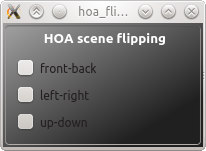
\includegraphics[width=0.3\columnwidth]{hoa_mirroring.png}
\caption{\lstinline'hoa_mirroring' plug-in under Linux jack-qt4. The check-boxes allows to select the mirror transformation : 'left-right', 'front-back' or 'up-down'.}
\label{fig:hoa_mirroring}
\end{figure}
\begin{figure}[!ht]
\centering
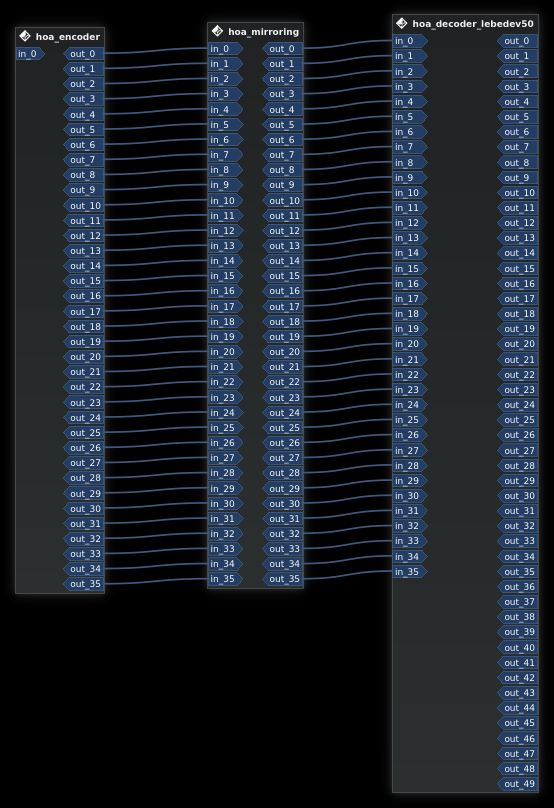
\includegraphics[width=0.5\columnwidth]{hoa_mirroring_claudia.png}
\caption{Example of \lstinline'hoa_mirroring' insertion between encoding and decoding steps, i.e. in Ambisonic domain.}
\label{fig:hoa_mirroring_claudia}
\end{figure}

\pagebreak
\subsubsection{hoa\_azimuth\_rotator}
\subsubsection{hoa\_beamforming\_to\_mono}
\subsubsection{hoa\_beamforming\_dirac\_to\_hoa}

\pagebreak
\subsection{Processing}
\subsubsection{Spherical\_VU\_Meter}
ambitools offers a Spherical VU-Meter developped with \textsc{Processing} language. A screen-shot is shown on Fig.~\ref{fig:spherical_vu_meter}. This tool allows to "see" where the sound energy is in space, instead of using classical in-line VU-Meter. You can zoom, pan and rotate the view of the meter while running. The \textsc{Faust} tools \lstinline'hoa_panning*' and \lstinline'hoa_decoder*' emit \textsc{OSC} messages on port UDP 5511. Those messages drive the spherical VU-Meter : loudspeakers size and color for the meter, and source position.
\begin{figure}[!ht]
\centering
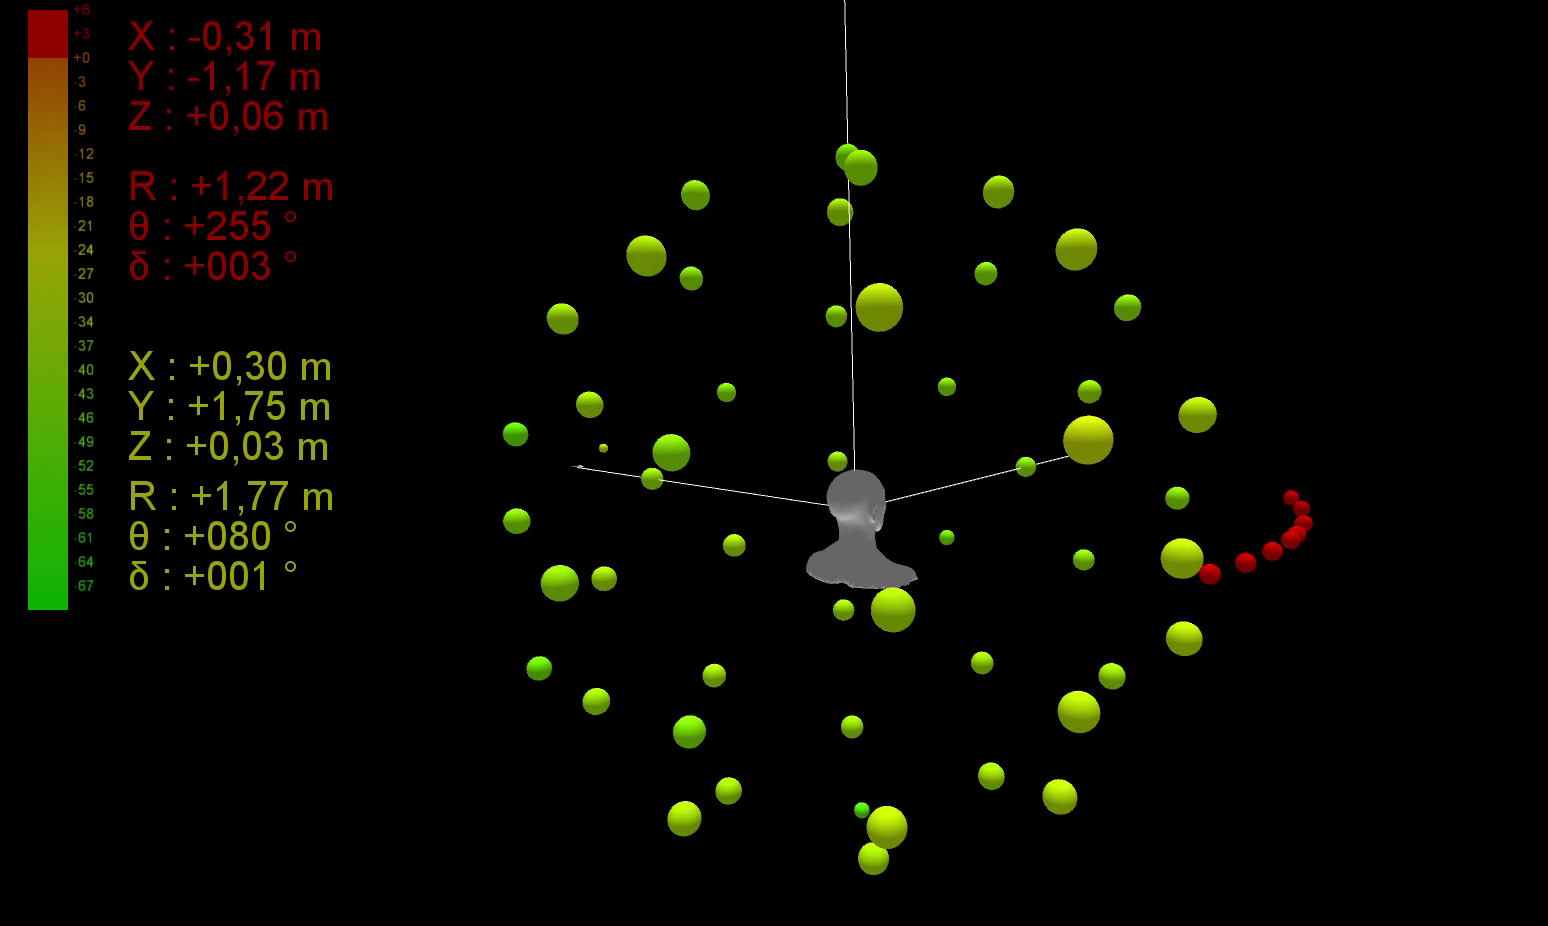
\includegraphics[width=\columnwidth]{spherical_vu_meter.png}
\caption{\lstinline'Spherical_VU_Meter' for a 50 loudspeaker Lebedev array and two virtual sources. Each loudspeaker is represented as a color ball with size and color proportional to RMS Level in dBFS. A scale in dBFS is displayed on the left of the screen. The virtual sources are represented as red an yellow dots. Their coordinates are displayed in Cartesian and spherical coordinates on the left. A grey manikin is standing in the middle of the array to indicates the front direction.}
\label{fig:spherical_vu_meter}
\end{figure}

\pagebreak
\subsection{Jconvolver}
\subsubsection{jconvolver\_mic*}
\subsubsection{hrir\_lebedev50}
%\section{Examples}
%\subsection{Flys flying around}
%\subsection{Record trajectories with Ardour}
\bibliography{These,ATIAM,Livres}
\bibliographystyle{apalike}

\end{document}
